%%%%%%%%%%%%%%%%%%%%%%%%%%%%%%%%%%%%%%%%%
% Beamer Presentation
% LaTeX Template
% Version 1.0 (10/11/12)
%
% This template has been downloaded from:
% http://www.LaTeXTemplates.com
%
% License:
% CC BY-NC-SA 3.0 (http://creativecommons.org/licenses/by-nc-sa/3.0/)
%
%%%%%%%%%%%%%%%%%%%%%%%%%%%%%%%%%%%%%%%%%

%----------------------------------------------------------------------------------------
%	PACKAGES AND THEMES
%----------------------------------------------------------------------------------------

\documentclass{beamer}

\mode<presentation> {

    % The Beamer class comes with a number of default slide themes
    % which change the colors and layouts of slides. Below this is a list
    % of all the themes, uncomment each in turn to see what they look like.

    %\usetheme{default}
    %\usetheme{AnnArbor}
    %\usetheme{Antibes}
    %\usetheme{Bergen}
    %\usetheme{Berkeley}
    %\usetheme{Berlin}
    %\usetheme{Boadilla}
    %\usetheme{CambridgeUS}
    %\usetheme{Copenhagen}
    %\usetheme{Darmstadt}
    %\usetheme{Dresden}
    %\usetheme{Frankfurt}
    %\usetheme{Goettingen}
    %\usetheme{Hannover}
    %\usetheme{Ilmenau}
    %\usetheme{JuanLesPins}
    %\usetheme{Luebeck}
    \usetheme{Madrid}
    %\usetheme{Malmoe}
    %\usetheme{Marburg}
    %\usetheme{Montpellier}
    %\usetheme{PaloAlto}
    %\usetheme{Pittsburgh}
    %\usetheme{Rochester}
    %\usetheme{Singapore}
    %\usetheme{Szeged}
    %\usetheme{Warsaw}

    % As well as themes, the Beamer class has a number of color themes
    % for any slide theme. Uncomment each of these in turn to see how it
    % changes the colors of your current slide theme.

    %\usecolortheme{albatross}
    %\usecolortheme{beaver}
    %\usecolortheme{beetle}
    %\usecolortheme{crane}
    %\usecolortheme{dolphin}
    %\usecolortheme{dove}
    %\usecolortheme{fly}
    %\usecolortheme{lily}
    %\usecolortheme{orchid}
    %\usecolortheme{rose}
    %\usecolortheme{seagull}
    %\usecolortheme{seahorse}
    %\usecolortheme{whale}
    %\usecolortheme{wolverine}

    %\setbeamertemplate{footline} % To remove the footer line in all slides uncomment this line
    %\setbeamertemplate{footline}[page number] % To replace the footer line in all slides with a simple slide count uncomment this line

    %\setbeamertemplate{navigation symbols}{} % To remove the navigation symbols from the bottom of all slides uncomment this line
}

\usepackage[export]{adjustbox}
\usepackage{graphicx} % Allows including images
\usepackage{booktabs} % Allows the use of \toprule, \midrule and \bottomrule in tables
\graphicspath{ {./figures/} }


% Insert title slides
\AtBeginSection[]{
  \begin{frame}
  \vfill
  \centering
  \begin{beamercolorbox}[sep=8pt,center,shadow=true,rounded=true]{title}
    \usebeamerfont{title}\insertsectionhead\par%
  \end{beamercolorbox}
  \vfill
  \end{frame}
}

%----------------------------------------------------------------------------------------
%	TITLE PAGE
%----------------------------------------------------------------------------------------

\title[ESS-NW/CAR]{ESS-NW/CAR } % The short title appears at the bottom of every slide, the full title is only on the title page

\author{ Leon Fernandez, Jonas Ekman, Fredrik Hyyrynen, Jacob Kimblad, Yini Gao and  Yifan Ruan} % Your name
\institute[KTH] % Your institution as it will appear on the bottom of every slide, may be shorthand to save space
{
    MF2063 \\ % Your institution for the title page
    \medskip

}
\date{December 10, 2018} % Date, can be changed to a custom date

\begin{document}

\begin{frame}
    \titlepage % Print the title page as the first slide
\end{frame}

\begin{frame}
    \frametitle{Overview} % Table of contents slide, comment this block out to remove it
    \tableofcontents % Throughout your presentation, if you choose to use \section{} and \subsection{} commands, these will automatically be printed on this slide as an overview of your presentation
\end{frame}

%----------------------------------------------------------------------------------------
%	PRESENTATION SLIDES
%----------------------------------------------------------------------------------------

\section{Introduction and background} 
\subsection{Autonomous vehicles}
\begin{frame}{Autonomous vehicles}
    \begin{figure}
        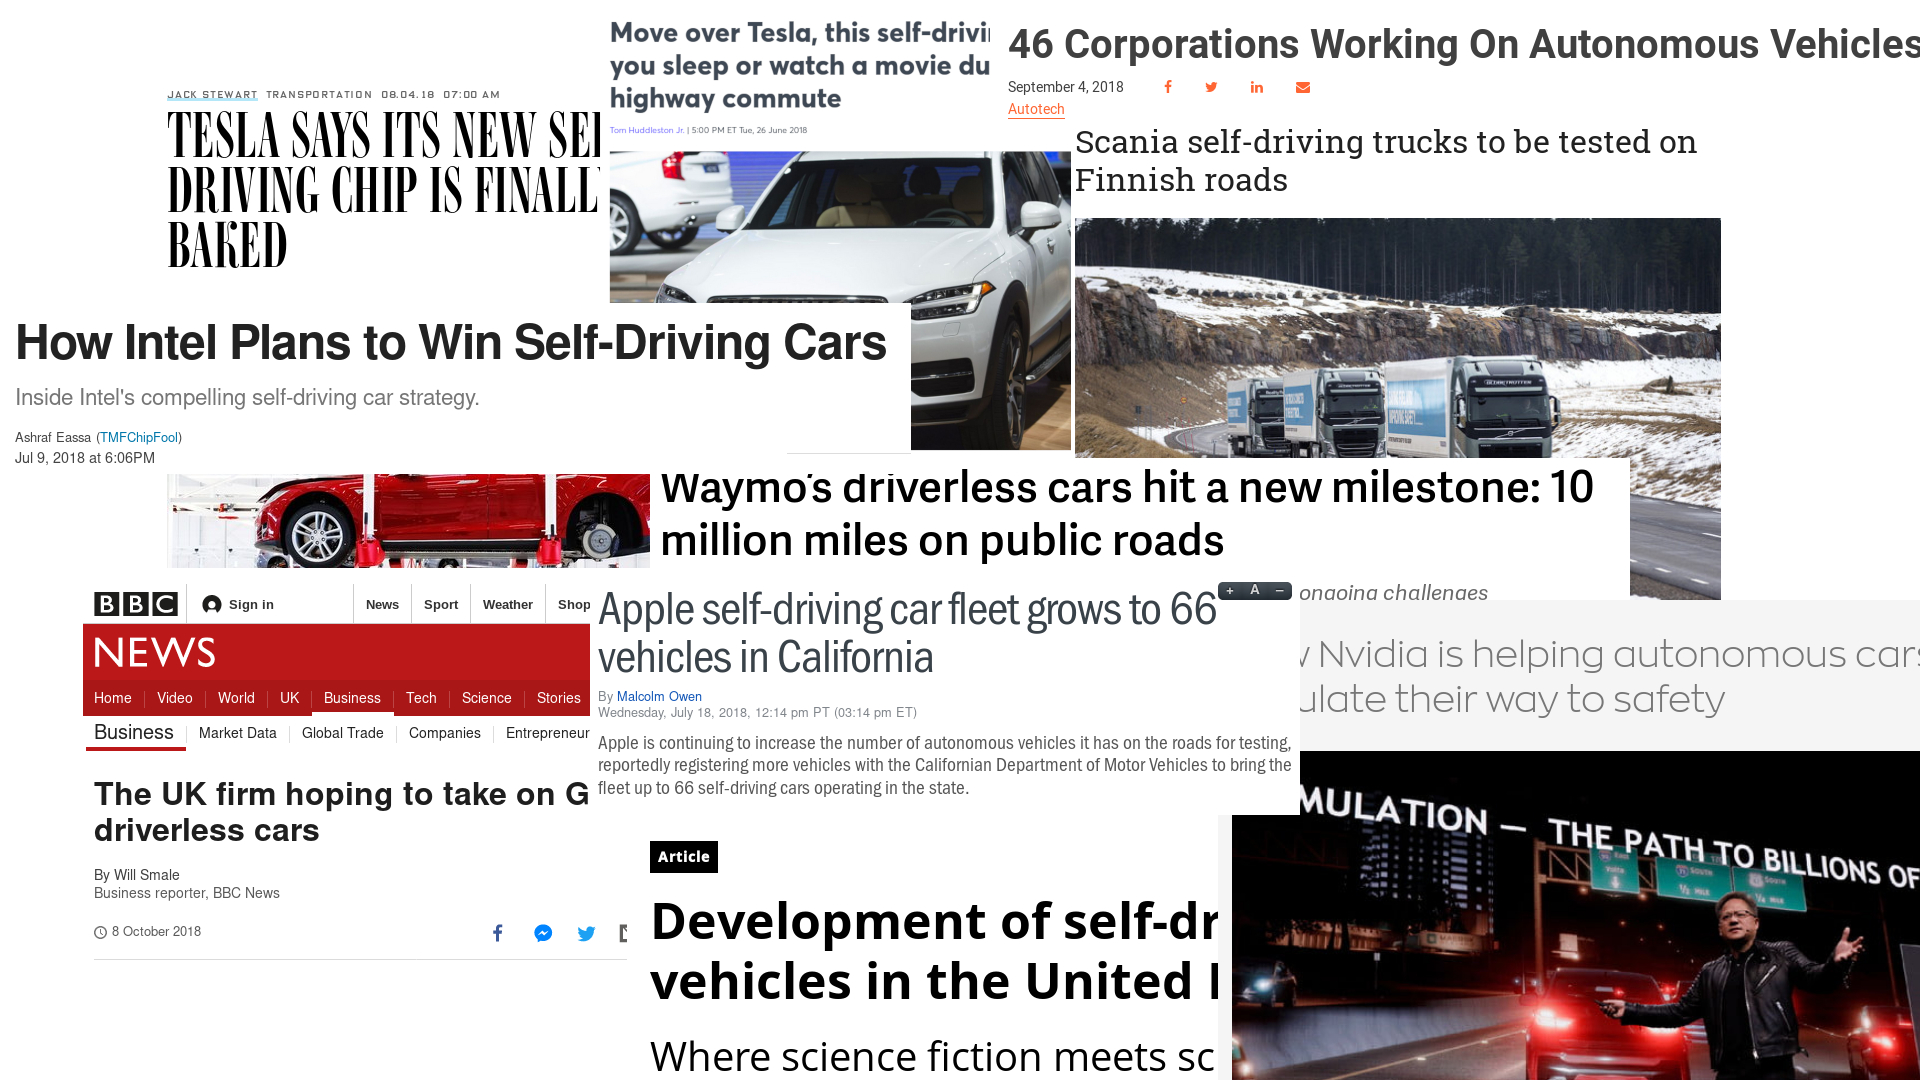
\includegraphics[width=1.1\linewidth]{articles.jpg}
    \end{figure}
\end{frame}

%------------------------------------------------
\begin{frame}{Autonomous vehicles}
    \begin{figure}
        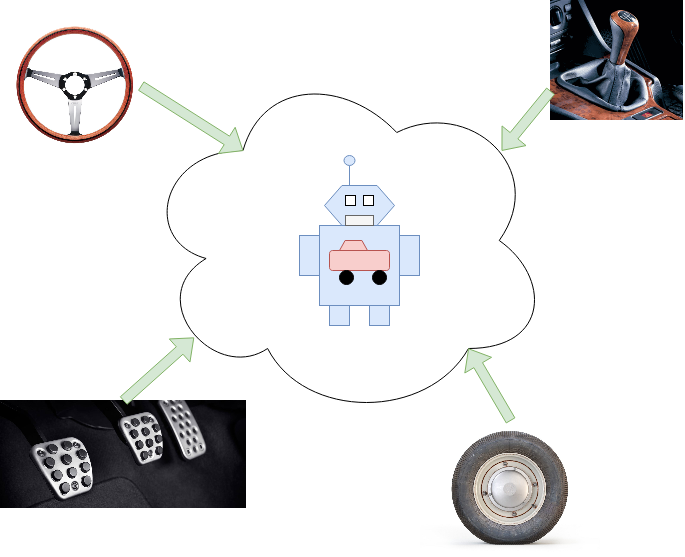
\includegraphics[width=0.7\linewidth]{driving.png}
    \end{figure}
\end{frame}

\begin{frame}{Autonomous vehicles}
    \begin{figure}
        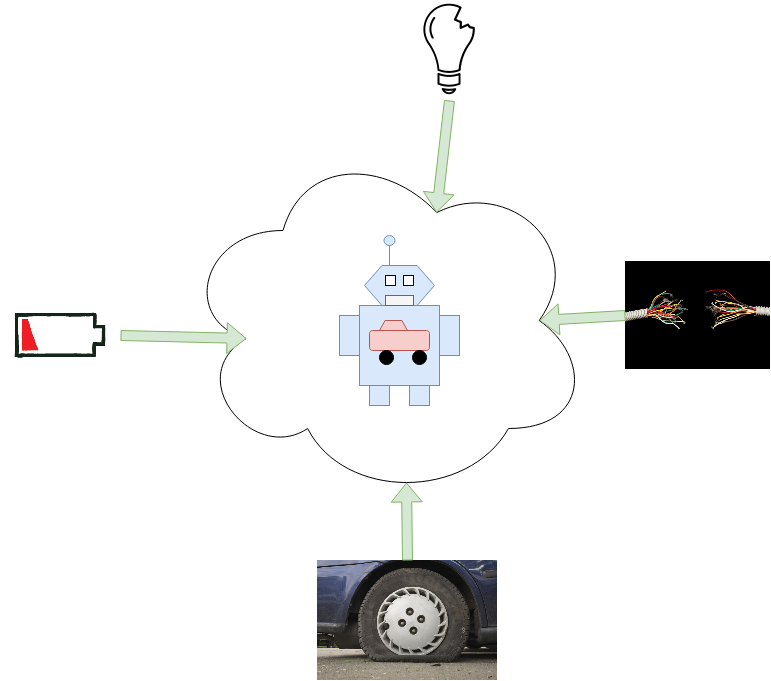
\includegraphics[width=0.7\linewidth]{monitoring.png}
    \end{figure}
\end{frame}

\begin{frame}{Autonomous vehicles}
    \begin{figure}
        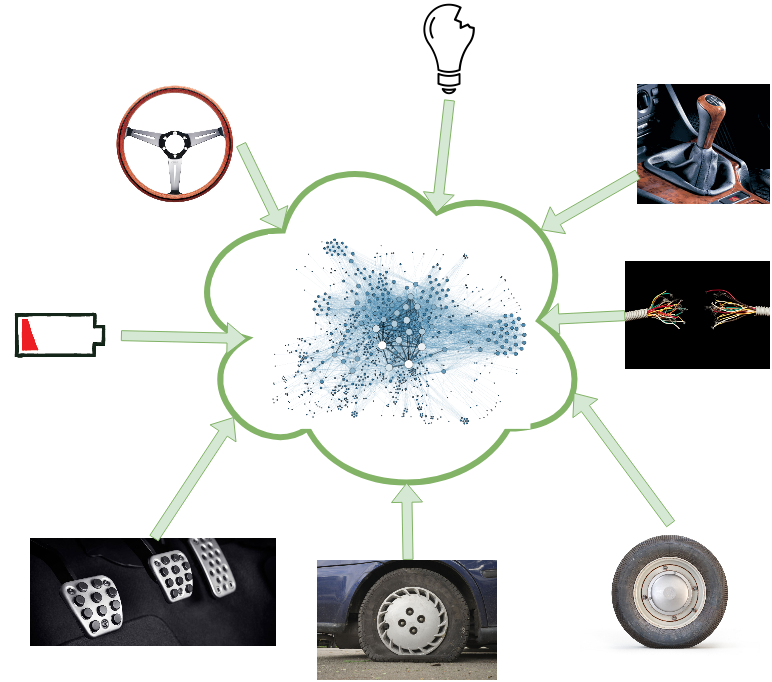
\includegraphics[width=0.7\linewidth]{networking.png}
    \end{figure}
\end{frame}


\subsection{Communication technologies}
\begin{frame}{The problem with existing communication technologies}
    \begin{itemize}
        \item Existing communication technologies between internal computers in cars:
            \begin{itemize}
                \item CAN (1 Megabit/s)
                \item LIN (19.2 Kilobit/s)
                \item FlexRay (10 Megabit/s)
            \end{itemize}
        \item Too slow for autonomous cars!
        \item Regular internet based technologies can be a solution for communication in cars.
        \item Wired ethernet speeds reach into the Gigabit/s range.
    \end{itemize}
    \begin{figure}
        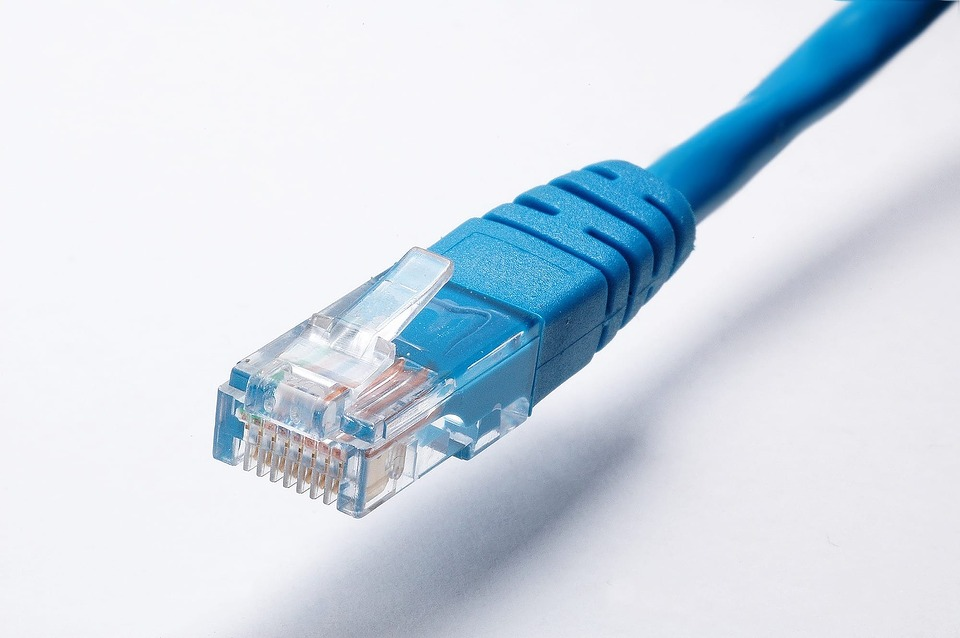
\includegraphics[width=0.3\linewidth]{ethernet_cable.jpg}
    \end{figure}
\end{frame}

\begin{frame}{The problem with existing communication technologies}
    \begin{figure}
        \includegraphics[width=0.7\linewidth]{congesting.png}
    \end{figure}
\end{frame}

\subsection{Software-Defined Networking}
\begin{frame}{Software-Defined Networking (SDN)}
    \begin{figure}
        \includegraphics[width=0.75\linewidth]{routing.png}
    \end{figure}
\end{frame}

\begin{frame}{Software-Defined Networking (SDN)}
    \begin{figure}
        \includegraphics[width=0.7\linewidth]{cooperating.png}
    \end{figure}
\end{frame}
%------------------------------------------------

\section{Our project}
\subsection{Goals}
\begin{frame}{Goals of the project}
    \begin{itemize}
        \item Produce a prototype of an SDN-based communication infrastructure for automotive vehicles.
        \item Produce a prototype of intelligent system monitoring and adaptation service for automotive vehicles.
        \begin{figure}
            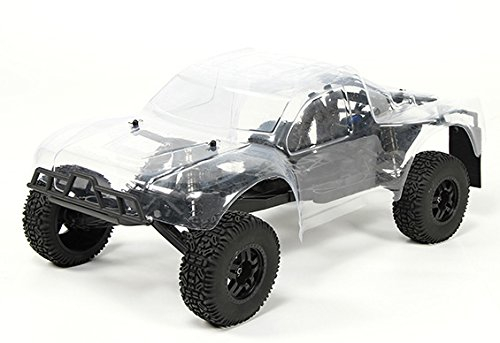
\includegraphics[width=0.5\linewidth]{turnigy_car.jpg}
            \caption{RC-car model kit used for the prototype}
        \end{figure}
    \end{itemize}
\end{frame}

%------------------------------------------------

\subsection{System architecture}
\begin{frame}{System architecture}
    \begin{figure}
        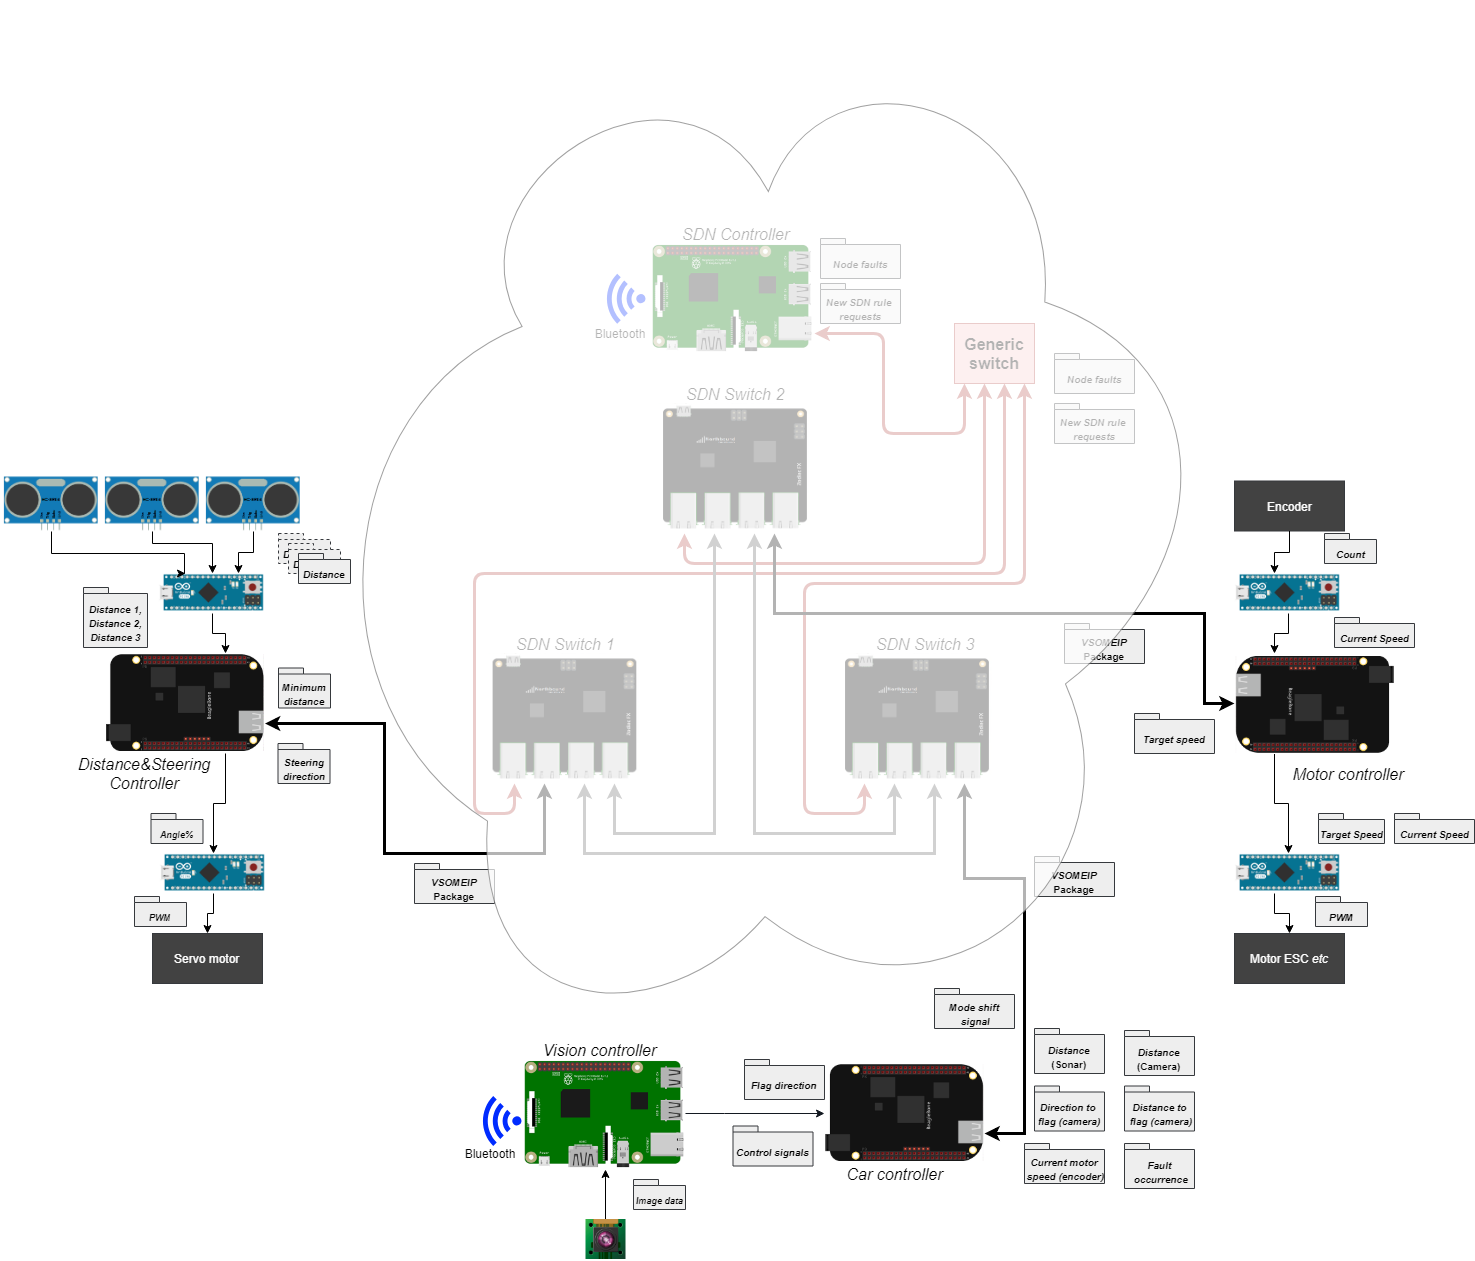
\includegraphics[width=0.83\linewidth]{network.png}
    \end{figure}
\end{frame}

%------------------------------------------------

\subsection{Implemented services}
\begin{frame}{Implemented services}
    \begin{itemize}
        \item Speedometer
        \item Cruise control
        \item Steering
        \item Object recognition
        \item Distance measurement
    \end{itemize}
    \begin{figure}
        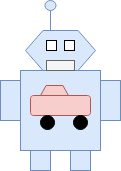
\includegraphics[width=0.2\linewidth]{robocar.png}
    \end{figure}
\end{frame}

\begin{frame}{Network surveillance}
    \begin{figure}
        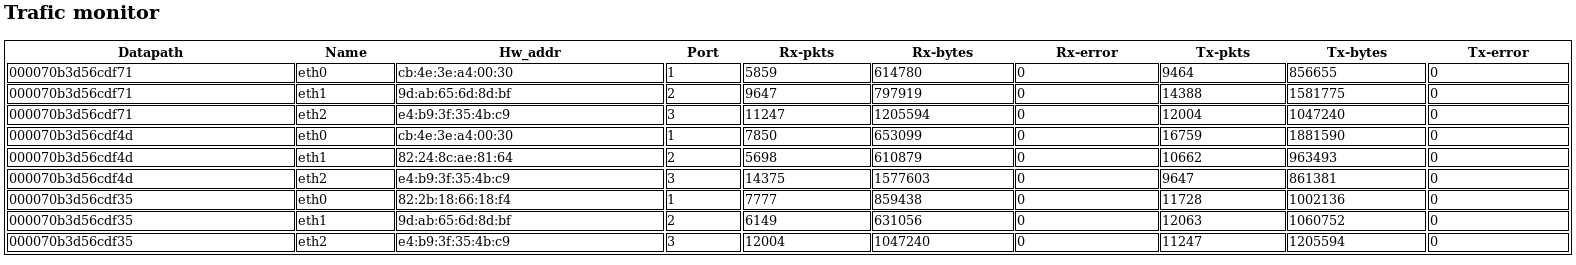
\includegraphics[width=1.05\linewidth]{netstat1.png}
    \end{figure}
    \begin{figure}
        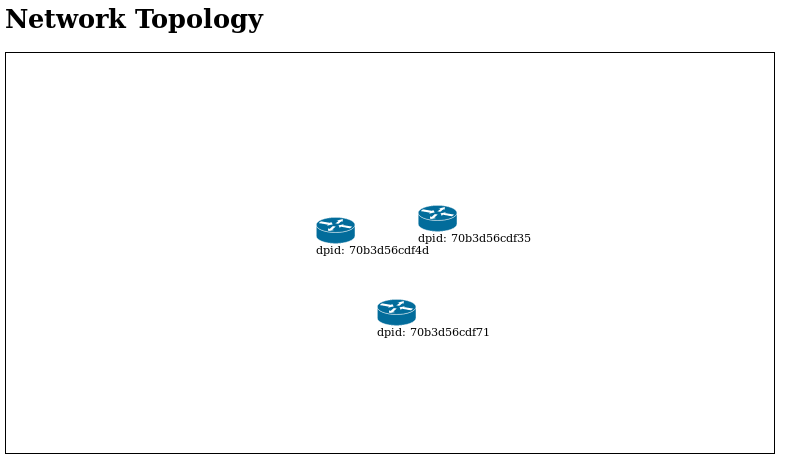
\includegraphics[width=0.6\linewidth]{netstat2.png}
        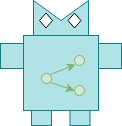
\includegraphics[width=0.2\linewidth]{robonet.png}
    \end{figure}
\end{frame}
%------------------------------------------------

\section{Summary}
\begin{frame}{Summary}
    \begin{itemize}
        \item Ethernet is a promising candidate for increasing demand on bandwidth for communication in autonomous cars
        \item Ethernet is not without problems, many of which a SDN can help to solve.
        \item SDN networks allow for safe communications on autonomous vehicles by being fast, adaptive and customisable
        \item Fault detection and failsafe behaviour is a \textbf{must} in autonomous vehicles.
    \end{itemize}

\end{frame}

%------------------------------------------------

\begin{frame}
    \Huge{\centerline{Come check out our DEMO in the}} 
    \Huge{\centerline{prototyping lab on floor 3!}} 
    \begin{figure}
        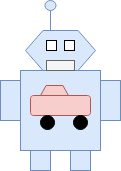
\includegraphics[width=0.2\linewidth]{robocar.png}
        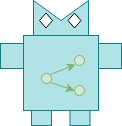
\includegraphics[width=0.2\linewidth]{robonet.png}
    \end{figure}
\end{frame}


%----------------------------------------------------------------------------------------

        \end{document}
